%!TEX TS-program = xelatex
\documentclass[]{friggeri-cv}
\usepackage{afterpage}
\usepackage{graphicx}
\usepackage{hyperref}
\usepackage{color}
\usepackage{pdfpages}
\usepackage{xcolor}
\hypersetup{
    pdftitle={},
    pdfauthor={},
    pdfsubject={},
    pdfkeywords={},
    colorlinks=false,       % no lik border color
   allbordercolors=white    % white border color for all
}
\addbibresource{bibliography.bib}
\RequirePackage{xcolor}
\definecolor{pblue}{HTML}{0395DE}

\begin{document}
\header{Donovan }{Riaño E.}
      {Student Computation Engineering }
      
% Fake text to add separator      
\fcolorbox{white}{gray}{\parbox{\dimexpr\textwidth-2\fboxsep-2\fboxrule}{%
.....
}}

% In the aside, each new line forces a line break
\begin{aside}
  \section{Tel \& Skype}
    +52 55-12-29-16-07
    live:driano7\_1
    ~
  \section{Emails}
    \href{mailto:donovanriano@gmail.com}{\textbf{donovanriano@}\\gmail.com}
    \href{mailto:driano7@outlook.com}{\textbf{driano7@}\\outlook.com}
    ~
  \section{Programming}
    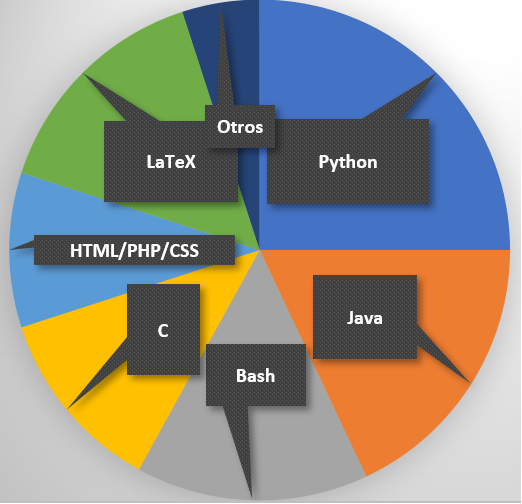
\includegraphics[scale=0.28]{L1.png}
    ~
  \section{OS Preference}
    \textbf{GNU/Linux}
\includegraphics[scale=0.40]{img/4stars.png}
    \textbf{Windows}
\includegraphics[scale=0.40]{img/3stars.png}
    \textbf{MacOS}
\includegraphics[scale=0.40]{img/3stars.png}
    ~
  \section{Languajes}
    \textbf{Spanish}
\includegraphics[scale=0.40]{img/5stars.png}
    \textbf{English}
\includegraphics[scale=0.40]{img/3stars.png}
    \textbf{French}
\includegraphics[scale=0.40]{img/1stars.png}
  ~
  \section{Personal Skills}
    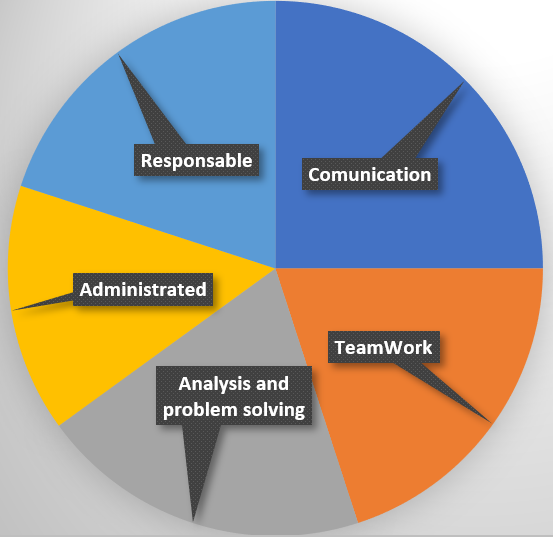
\includegraphics[scale=0.28]{H2.png}
    ~
\end{aside}

\section{Education}
\begin{entrylist}
\entry
    {2017-Now}
    {5th Semester of Bachelor}
    {UNAM, Facultad de Ingeniería}
    {Most Important Subjects: Objected-Oriented Programming, Artificial Intelligence(IA), Data Bases, Secure Data Networks,     
    Formal Languages and Automatas, Data Structure and Algorithms (I and II).
    %\emph{Title of the Thesis: "A Handoff Algorithm based on Link Quality Prediction for Mass Transit Wireless Mesh Networks"      .}\\
    %\emph{Relators: Prof. Enzo Mingozzi, Ing. Carlo Vallati, Prof. Luciano Lenzini.}\\
    }
\entry
    {Winter 2018}
    {Extracurricular Course}
    {Anexo de Ingeniería, UNAM, CDMX}
    {La Integral, Métodos de Integración y Aplicaciones\\
    Course Purpouse: aplications of Integrals, 15 hours.}

\entry
    {Summer 2019}
    {Extracurricular Course}
    {Anexo de Ingeniería, UNAM, CDMX}
    {Python \& Machine Learning Avanzado\\
    Course Purpouse: examples, implementations and uses of Artificials Neuronal Networks with tool Colab, 10 hours.}

\end{entrylist}

\section{Experience}
\begin{entrylist}
  \entry
    {Summer 2018}
    {CAE IECM}
    {Aniceto Ortega 917, Benito Juárez, CDMX}
    {Election Assistant Trainer in Elections 2018.\\}
  
\end{entrylist}


%\section{Certifications}
%\begin{entrylist}
%  \entry
%    {02/2013}
%    {Intro to Computer Science}
%    {Udacity. E-learning}
%    {\emph{Building a Python Search Engine}}
%\end{entrylist}

\section{Proceedings}
Riaño D., Molero-Castillo G. Vázquez Mena A., Bárcenas E.(2019)\\
\textbf{Tratamiento de Expresiones Regulares en la Privacidad de Navegadores Web}\\
\emph{Conferencia Internacional de Investigación e Innovación en Ingeniería de Software (CONISOFT’19) , Facultad de Ingeniería, UNAM, CDMX, México.}

\section{Journals}

Riaño D., Molero-Castillo G. Vázquez Mena A., Bárcenas E.(2019)\\
\textbf{Tratamiento de Expresiones Regulares en la Privacidad de Navegadores Web}\\
\emph{Abstraction and Application (A\&A), Autonomous University of Yucatan, UADY, Mérida Yucatán, November, 2019.}
\\
\section{Another Information}

\emph{Word Processor \LaTeX. \\ }
\emph{Human Signal Processing with Python (Libraries: NumPy, SciPy, Stats, MatplotLib,Pandas).\\}
\emph{Graphing Probability Distributions with R and python (MatplotLib, Seaborn, SciPy, Numpy,Stats).\\}
\emph{Notions: , Graphic Interfaces in Java, Optical Character Recognition (OCR) with Tesseract and OpenCV in Python, API Speech Recognition of Google in Python. \\}
\emph{Data Bases in PHP myAdmin, Oracle and Microsoft SQL Server Management Studio 2016.}
\emph{Software: Word, Excel, PowerPoint, LibreOffice, SublimeText, Brackets, Visual Studio, Bash Linux.\\ }
%\emph{ }
\\
\begin{flushleft}
\emph{September 6, 2019; Donovan Riaño Enriquez}
\end{flushleft}

%\begin{flushright}
%\emph{Donovan Riaño Enriquez}
%\end{flushright}

\clearpage


\includepdf[pages={1}]{Comp.pdf} 
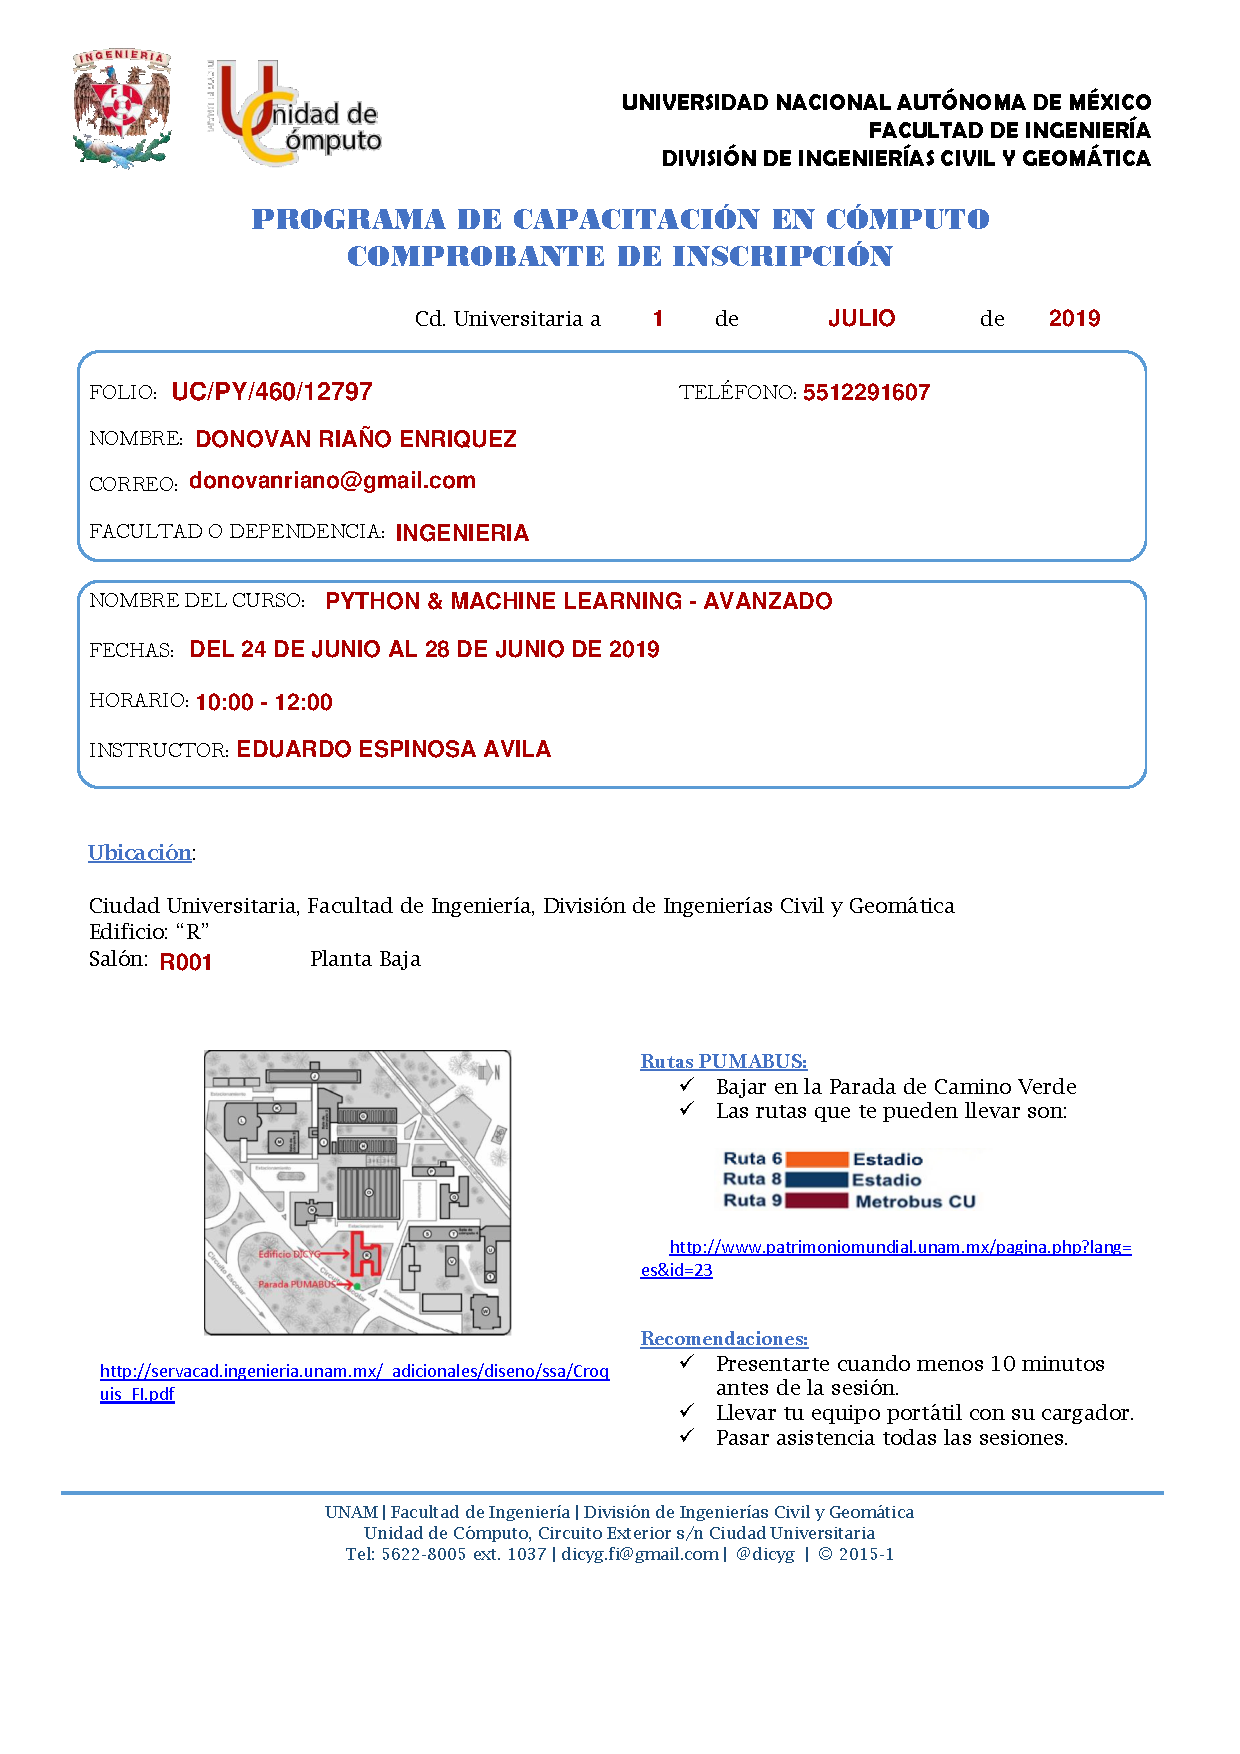
\includepdf[pages={1}]{machine.pdf} 
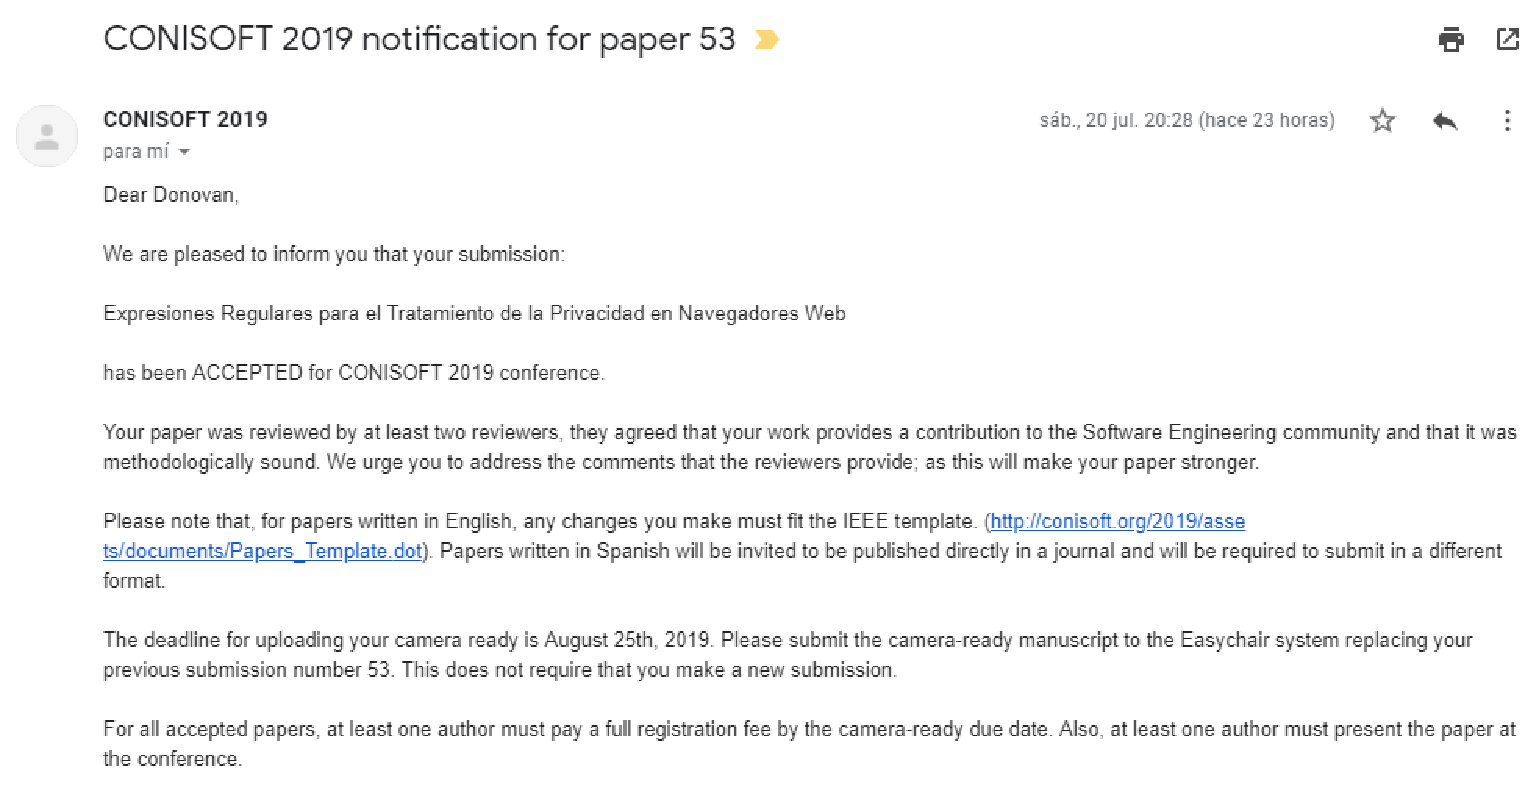
\includepdf[pages={1}]{aceptacion.pdf} 

\includepdf[pages={1}]{A&A.pdf}
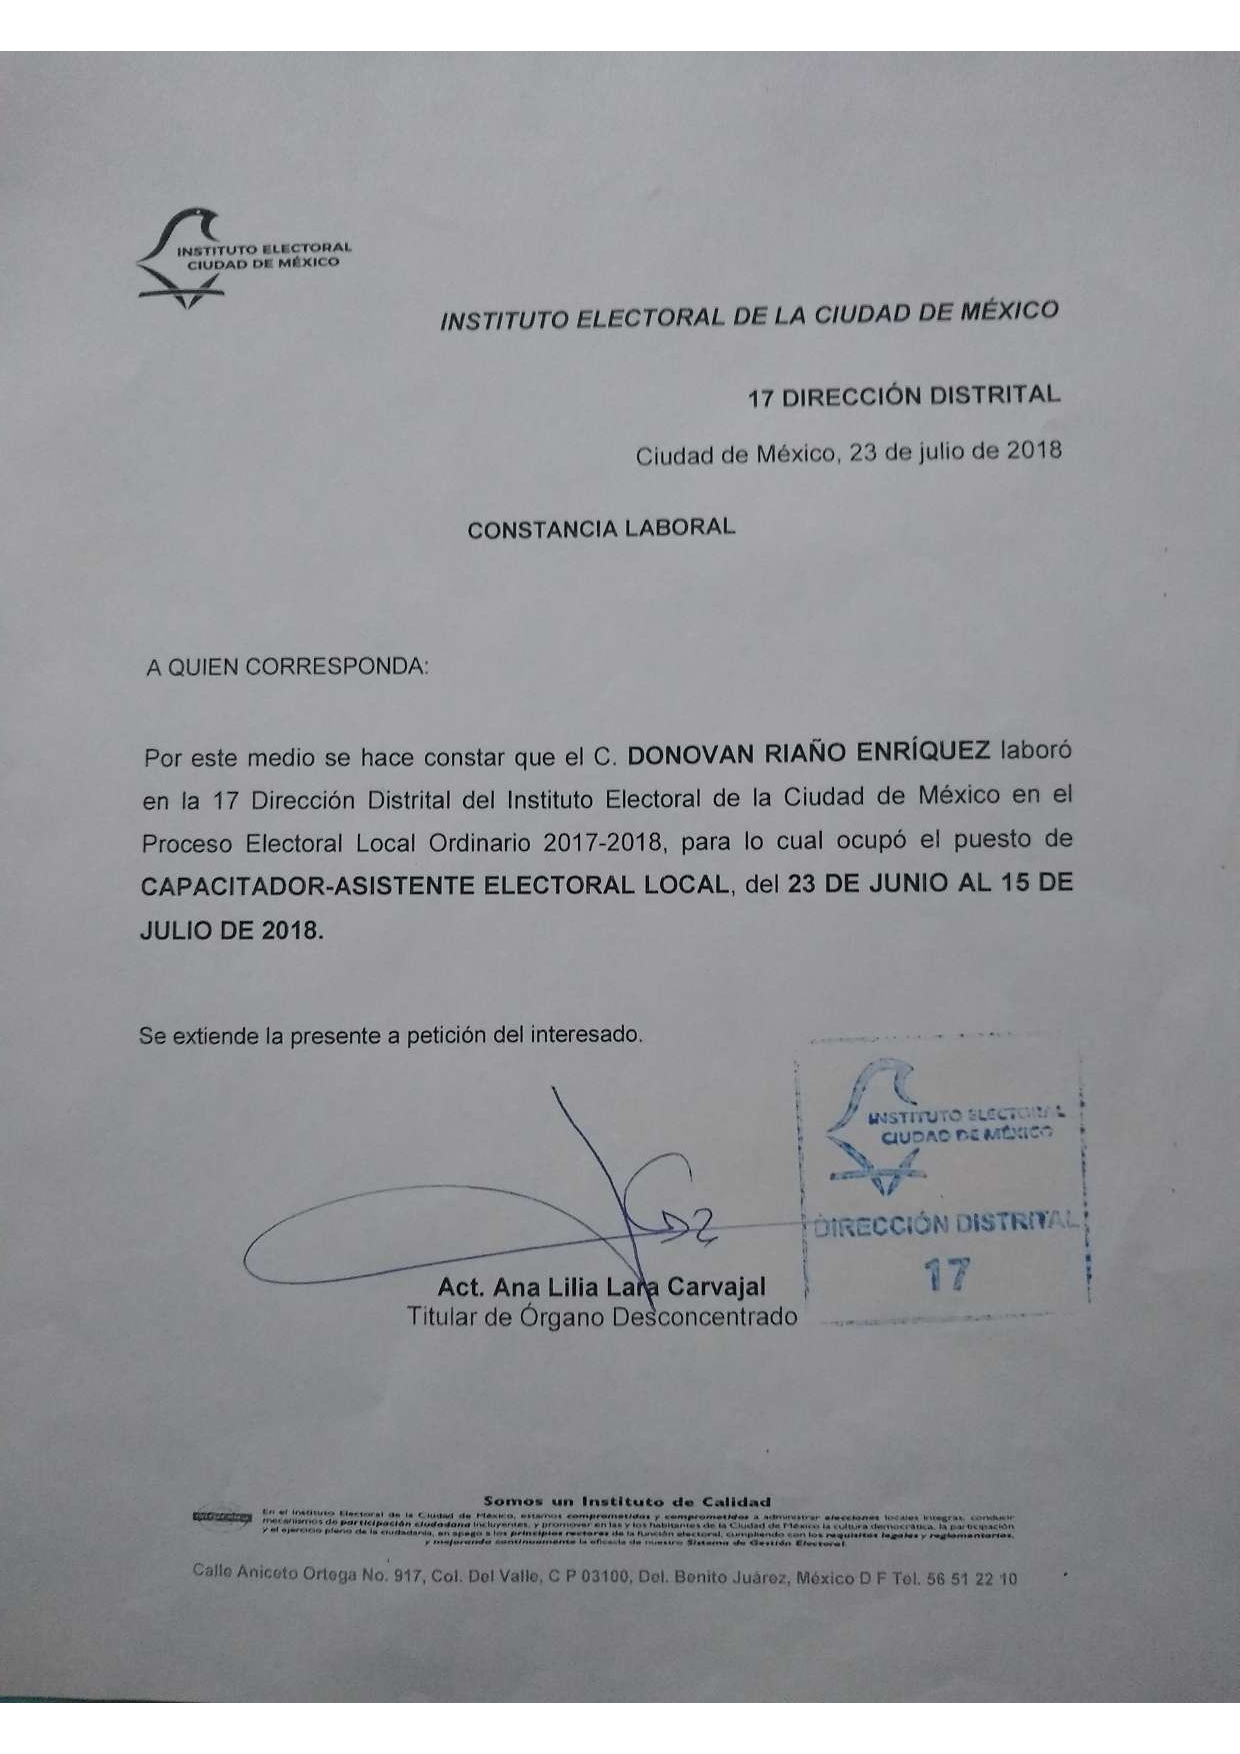
\includepdf[pages={1}]{Iecm.pdf} 


%%% This piece of code has been commented by Karol Kozioł due to biblatex errors. 
% 
%\printbibsection{article}{article in peer-reviewed journal}
%\begin{refsection}
%  \nocite{*}
%  \printbibliography[sorting=chronological, type=inproceedings, title={international peer-reviewed conferences/proceedings}, notkeyword={france}, heading=subbibliography]
%\end{refsection}
%\begin{refsection}
%  \nocite{*}
%  \printbibliography[sorting=chronological, type=inproceedings, title={local peer-reviewed conferences/proceedings}, keyword={france}, heading=subbibliography]
%\end{refsection}
%\printbibsection{misc}{other publications}
%\printbibsection{report}{research reports}

\end{document}
